\documentclass[thesis=bachelor,faculty=cb]{hsmw-thesis}
\usepackage{listings}
\usepackage{xcolor}
\usepackage{float}
\usepackage{amsfonts}
\title[Research on the certificate-based updating of embedded control systems]{Untersuchungen zur zertifikatsbasierten Aktualisierung von verteilten Steuerungssystemen}
\author{Marc}{Ulbricht} 
%<signatur-schildbach.pdf>
\submissiondate{2022}[8][4]
\courseofstudy[Applied Computer Science]{Angewandte Informatik}
\seminargroup{IF17wI-B}
\examiner[Prof. Dr.-Ing.]{Thomas Beierlein}
\addexaminer{Andreas Weger}[M.Sc.]
\abstract{In dieser Bachelorarbeit soll ein System, welches die Authentizität und Unversehrtheit einer Firmwareaktualisierung vor Installation auf dem Zielgerät sicherstellt, theorisiert und umgesetzt werden.
	Hierfür werden Verfahren herangezogen, welche auf möglichst lange Sicht sicher bleiben, aber gleichzeitig immer größer werdende Firmwarepakete trotzdem effizient verarbeiten sollen.
	Dabei ist zu priorisieren, dass möglichst wenig Änderungen am Zielgerät vorgenommen werden, da sich diese im bereits ausgelieferten Zustand befinden
	Des Weiteren soll sich der bisherige Ablauf einer Aktualisierung nicht merkbar verändern.}
\lstset{basicstyle=\ttfamily,
	keywordstyle=\color{blue}\ttfamily,
	showstringspaces=false,
	stringstyle=\color{orange}\ttfamily,
	commentstyle=\color{red}\ttfamily,
	morecomment=[l][\color{magenta}]{\#},
	breaklines=true
}
\begin{document}
\chapter{Einleitung}
Sicherheit und vor allem Sicherheit im Internet ist eines der großen Themen dieser Zeit, vor allem jetzt, da immer mehr Geräte und nicht nur der Heimcomputer mit dem Internet verbunden sind. Bei einer Firma wie \href{https://iseg-hv.com/de/}{Iseg}, welche Hochspannungsversorgungen für Wirtschaft und Industrie herstellt ist Sicherheit um so wichtiger. Erst vor kurzem wurde eine Sicherheitslücke \cite{0Day} im Diagnose-Tool von Microsoft \enquote{Office Microsoft Support Diagnostic Tool (MSDT)} entdeckt.
Das Öffnen eines Word-Dokumentes und das leichtfertige Deaktivieren der \enquote{geschützten Ansicht} reicht dem Angreifer bereits aus, um Code nachzuladen und PowerShell-Code auszuführen.
Der Angreifer kann sich so möglicherweise Rechte verschaffen und das ganze System übernehmen. Welche Auswirkungen solch ein Zugang bei Iseg haben könnte ist leicht vorstellbar.
\newline
Deshalb müssen externe Dateien wie zum Beispiel Firmwareaktualisierungen verifiziert werden, bevor sie am Gerät Verwendung finden können.
\newpage
\section{Aufgabenstellung}
Ziel dieser Bachelorarbeit ist die Planung und Entwicklung einer Softwarelösung, welche die von der Firma \textit{Iseg} bereitgestellten Firmwareaktualisierungen signiert und verifiziert. Die Updates sollen vor dem Verteilen signiert werden und vor der Installation automatisch auf Echtheit und Unversehrtheit geprüft werden. Dabei soll es trotzdem möglich bleiben ein Update auch ohne gültige Verifikation durchzuführen, falls ein Fehler beim Verifizieren auftreten sollte, oder sich die Softwarelösung auf dem Gerät durch z.B. Alter des Gerätes nicht umsetzen lässt und keine Möglichkeit zum Verifizieren besteht.
\noindent
Hier wird dem Endkunden durch entsprechendes visuelles Feedback die Möglichkeit gegeben werden, zu entscheiden, ob und wie mit dem Update weiter verfahren wird. Dies soll allerdings die einzige mögliche merkbare Abweichung vom derzeitigen Aktualisierungsprozess sein.
Des Weiteren sind die Zielgeräte bereits ausgeliefert, daher ist ein Weg zu finden, die Softwarelösung möglichst einfach zu verteilen. 
Zu Beginn soll aber zunächst ein geeignetes Signaturverfahren erörtert werden, welches möglichst große Sicherheit bietet, ohne merklich die Geschwindigkeit eines Updates zu mindern.
\chapter{Grundlagen}
Dieses Kapitel gibt einen Einblick in die theoretische Grundlagen von Signaturverfahren. Dies soll vor allem dazu dienen, die Gründe hinter der \\ Entscheidung für ein Verfahren besser nachvollziehen zu können.
\section{Digitale Signaturen}
Digitale Signaturverfahren sind sogenannte Asymmetrische Kryptosysteme, auch \enquote{Public-Key-Verfahren} genannt. So erstellt ein Benutzer mithilfe eines mathematischen Verfahrens, worin sich die einzelnen Signaturverfahren unterscheiden, ein Schlüsselpaar aus einem geheimen und einem öffentlichen Schlüssel. Diese sollen in dieser Arbeit fortan \enquote{private-key} und \enquote{public-key} heißen. Mithilfe des private-key kann der Benutzer seine Daten eindeutig signieren. Der public-key dient dazu diese Signatur zu prüfen und kann den Benutzer somit als ursprünglichen Besitzer der Daten authentifizieren. 
\begin{figure}[H]
	\centering
	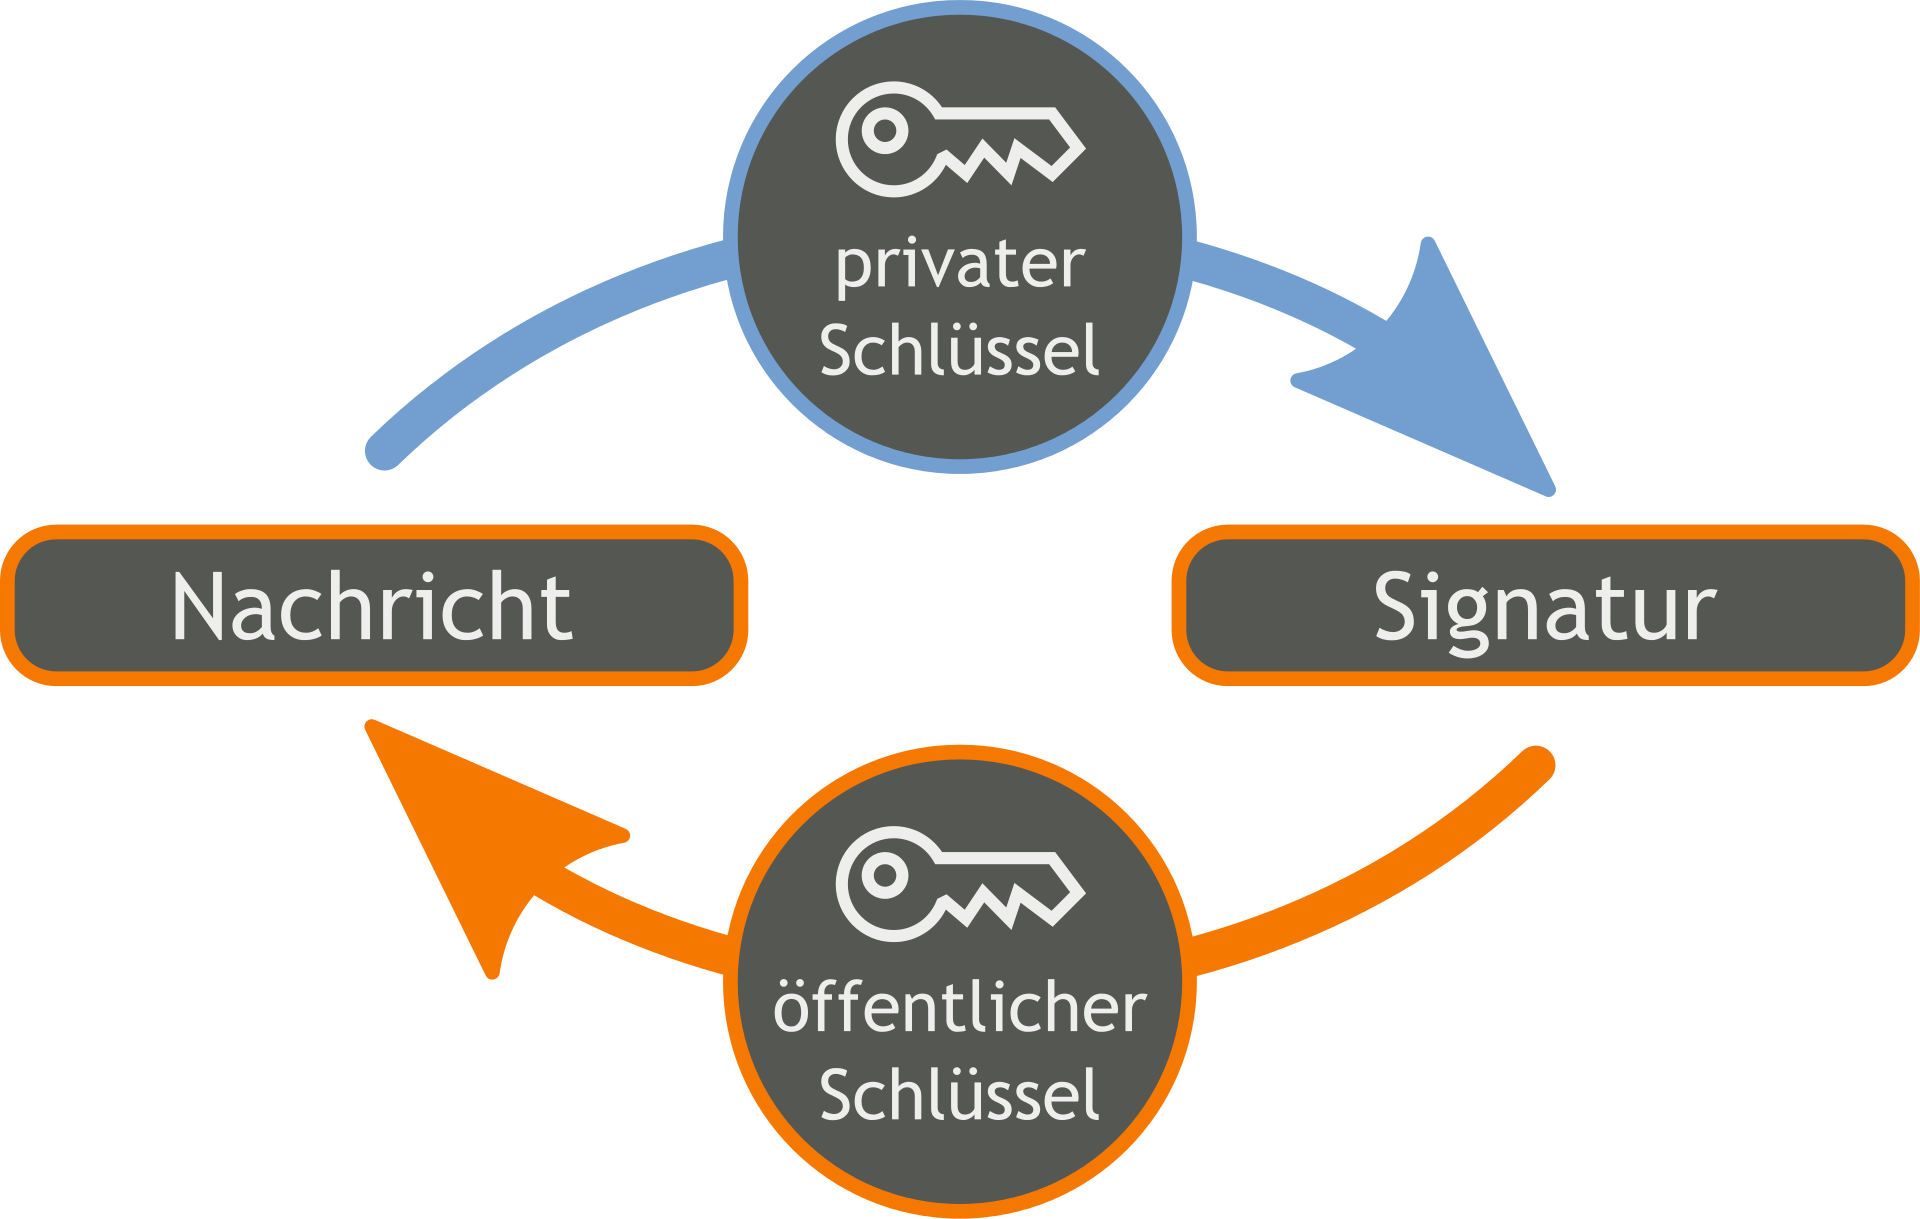
\includegraphics[scale=0.09]{images/Orange_blue_digital_signature_de.svg.png}
	\caption{Simplifizierte Veranschaulichung zu Signaturverfahren}{Quelle: \url{ https://upload.wikimedia.org/wikipedia/commons/2/29/Orange_blue_digital_signature_de.svg}}
\end{figure}
Darin liegt auch der Vorteil eines Asymmetrischen Kryptosystems, Sender und Empfänger müssen vorher kein gemeinsames Geheimnis ausmachen, da nur eine Partei den Ursprung und die Echtheit ihrer Daten darlegen will. Somit lassen sich zwar keine sensiblen Daten sicher versenden, aber dies wäre auch nicht zielführend für diese Arbeit. Digitale Signaturverfahren eignen sich dagegen sehr gut, da die Firmwareaktualisierungen der Firma \textit{iseg} auch öffentlich zugänglich sind und nur ihre Authentizität und Unversehrtheit vor der Installation nachgewiesen werden muss. \\
\\[1cm]
In den folgenden Teilkapiteln sollen nun die mathematischen Grundlagen der Schlüsselerzeugung der einzelnen Verfahren aufgezeigt werden.
\\[1cm]´
\section{RSA}
RSA ist ein asymmetrisches Kryptographieverfahren, welches 1978 von Ronald Rivest, Adi Shamir und Leonard Adleman veröffentlicht wurde. Aus ihren Nachnamen erschließt sich hierbei auch der Name des Verfahrens "RSA".
\\[1cm]
Für dieses Verfahren werden ein public-key und ein private-key generiert. Der public-key besteht dabei aus dem RSA-Modul $n$ sowie dem Verschlüsselungsexponenten $e$. Der private-key enthält ebenfalls $n$ und den Entschlüsselungsexponenten $d$.
Die Namen der Exponenten scheinen unsinnig, da beim Signieren der private-key verwendet wird. Dies hat den Grund, dass das Signieren die Operationen des Verschlüsselns einer Nachricht in umgekehrter Reihenfolge durchführt. So wird 
beim Verschlüsseln mit dem public-key agiert.
\\[1cm]
Für das Erstellen der Schlüssel werden zunächst zwei große zufällige Primzahlen $p$ und $q$ generiert, für welche $p \neq q$ gilt. Der RSA-Modul $n$ lässt sich nun als $n = p \times q$ berechnen. Außerdem wird \begin{math}\phi(n) = (p-1)\times(q-1) \end{math} berechnet.
$\phi()$ meint die Eulersche $\phi$-Funktion, welche einer natürlichen Zahl $n$ die Anzahl aller natürlicher Zahlen von $1$ bis $n$, welche zu $n$ teilerfremd sind, zuordnet. Hierbei handelt es sich um einen Spezialfall, da $p$ und $q$ Primzahlen sind. Somit wäre $q$ zu den Zahlen von $1$ bis $q-1$ teilerfremd und $\phi(q)$
lässt sich als $q-1$ darstellen. Wird dies auch bei $p$ angewandt ergibt sich für $\phi(n)$ die oben genannte Definition $\phi(n) = (p-1) \times (q-1)$. Danach wird der Verschlüsselungsexponent $e$ so gewählt, dass $e \in \mathbb{N}$, $1 < e < \phi(n)$ gilt und dass $e$ und $\phi(n)$ teilerfremd
sind. Der public-key ist somit berechnet und lässt sich als folgendes Tupel $(n, e)$ darstellen. 
\\[1cm]
Für den private-key fehlt nun noch der Entschlüsselungsexponent $d$, welcher sich aus $e \times d = 1 ( \mod \phi(n))$ berechnen lässt, vorausgesetzt $d \in \mathbb{N}$ und $d$ erfüllt die Vorgabe $1 < d < \phi(n)$.
Der private-key $(n, d)$ ist einsatzbereit, nun sollten sicherheitshalber $p$, $q$ und $\phi(n)$ gelöscht werden um mögliche Spuren von public und private-key zu verwischen. Eine Nachricht $m$ soll nun signiert werden. Zunächst wird ein Hash der Nachricht ($Hash(m)$) erstellt, da so die Größe der Nachricht keinen
Einfluss auf die Dauer des Signierens hat. Die Signatur $s$ berechnet sich nun als $s = (Hash(m))^{d} \mod n$ und kann zusammen mit dem public-key und der eigentlichen Nachricht dem Empfänger übermittelt werden. Der Empfänger berechnet nun $v = s^{e} \mod n$ und ermittelt selbst $Hash(m)$ der
originalen Nachricht. Stimmen $v$ und $Hash(m)$ überein besteht eine sehr hohe Chance, dass die Nachricht echt ist. Ihre Integrität und Authentizität sind sichergestellt. Die Sicherheit des RSA Verfahrens ist durch die Unkenntnis von $\phi(n)$ gegeben, so kann der Angreifer nicht einfach
den private-key reproduzieren. $\phi(n)$ lässt sich mit dem Wissen um  $p$ und $q$ über den vorher gezeigten Speziallfall einfach berechnen, ist jedoch ohne diese extrem Zeitaufwendig und unsinnig für einen Angreifer. Seine größte Chance liegt im Faktorisieren von $n$ in $p$ und $q$, hierfür sind jedoch auch
noch keine effizienten Algorithmen bekannt. Dies nennt man auch eine Einwegfunktion, da die Berechnungen nur in eine Richtung einfach durchzuführen sind. 
\section{Ed25519}
Ed25519 basiert auf EdDSA (Edwards-curve Digital Signature Algorithm) und wird im RFC 8032\cite{ed25519} genau beschrieben. Ursprünglich wurde Ed25519 im Wissenschaftlichen Aufsatz \enquote{High-speed high-security signatures} \cite{ed25519_paper} von   Daniel J. Bernstein, Niels Duif, Tanja Lange, Peter Schwabe und Bo-Yin Yang vorgestellt.
\\[1cm]
Ed25519 nutzt relativ kleine Schlüsselgrößen mit einem 32-Byte private-key, einem 32-Byte public-key uind einer 64-Byte Signatur und bietet trotzdem mit 128-Bit (Aufwand: \begin{math}O(2^{128})\end{math}) ein hohes Level an Sicherheit.
\\[1cm]
Schwere Fassung\footnote{\url{https://datatracker.ietf.org/doc/html/rfc8032\#section-5.1}}
Simplere Fassung\footnote{\url{https://wizardforcel.gitbooks.io/practical-cryptography-for-developers-book/content/digital-signatures/eddsa-and-ed25519.html}}
\newpage
\section{Vorstellung Iseg Updateverfahren}
\chapter{Evaluation Signaturverfahren}
\section{Vergleich Ed25519 und RSA}
\section{Vergleich Ed25519 und andere elliptische Kurven}
z.B. Ed448, weniger gegebene Bibliotheken zum implementieren, aber höhere Sicherheit
\section{Fazit/Entscheidung}
Ed25519 theoretisch schnellere Performance als RSA, bei gleicher Sicherheit und kleineren Schlüsselgrößen
\chapter{Implementierung}
\section{Python}
Zu Beginn der Arbeit wurde eine mögliche Umsetzung des Signatur- und Verifizierungsverfahrens in Python angestrebt. Eine mögliche Lösung hierfür fand sich in {\href{https://pypi.org/project/PyNaCl/}{PyNaCl}. PyNaCl bietet eine Python Anbindung zur \href{https://github.com/jedisct1/libsodium}{libsodium} Bibliothek, wobei es sich um einen portablen fork der \href{https://nacl.cr.yp.to/}{NaCl} (Networking and Cryptograhpy library) handelt. Somit ermöglicht PyNaCl die Verwendung des Ed25519-Signaturverfahrens in Python. Nach ersten Versuchen wurden die Arbeiten an dieser Implementierung jedoch eingestellt, da es sich herausstellte, dass ein Echtwelteinsatz sehr unwahrscheinlich sein wird. PyNaCl fordert eine Python Version von 3.6 oder höher, wobei auf den Geräten von Iseg derzeit maximal Python 3.5 vorzufinden ist. Ein mögliches Upgrade der Python Version wäre möglich, hat aber derzeit keine Priorität. 
	\\[1cm]
	Es ist unklar, ob sich ein weiterer Blick in PyNaCl lohnt, falls Python auf den Iseg Geräten geupdated werden sollte. Python unterliegt dem Stigma, langsamere Ausführungszeiten zu haben, da Python-Code erst während der Laufzeit interpretiert wird. Welche Auswirkungen dies genau auf das Verifizieren einer Signatur hat, lässt sich nicht vorher sagen. Somit bleibt diese Möglichkeit in Zukunft offen, es muss aber vorher getestet werden, ob überhaupt ein Zeitersparnis möglich ist und diese Implementierung sinnig wäre.
	\section{C}
	Implementierungen von Ed25519 wurden ursprünglich\footnote{\url{https://ed25519.cr.yp.to/software.html} Stand: 07.07.2022} in Assembler für amd64 Architektur und in C bereitgestellt. Diese wurden im SUPERCOP\footnote{\url{https://bench.cr.yp.to/supercop.html} Stand: 07.07.2022} toolkit verwendet.
	SUPERCOP wird eingesetzt, um die Leistungsfähigkeit verschiedenster Kryptografiealgorithmen auf unterschiedlicher Hardware zu testen.
	Im Zuge dessen wurde die alte C Implementierung \enquote{ref} verbessert und eine weitere Implementierung namens \enquote{ref10} entwickelt, welche bessere Leistung verspricht. Eine portable Implementierung\footnote{\url{https://github.com/orlp/ed25519} Stand: 07.07.2022}, welche auf dieser \enquote{ref10} Implementierung basiert, wurde für dieses Projekt verwendet. Die Anwendung soll nun vorgestellt werden.
	\\[1cm]
	Wir definieren als unsigniertes character-array einen 32-Byte seed, einen 32-Byte public-key, einen 64-Byte private-key und eine 64-Byte Signatur. Die größes des private-keys ist dabei unterschieldich zur Definition in 2.4, da die Implementierung anders damit umgeht. Zunächst wird der seed zufällig generiert (zum Beispiel unter Linux mit der Hilfe von /dev/urandom). Danach soll die zu signierende Nachricht eingelesen werden, was in diesem Fall die Firmwareaktualisierung darstellt. Die Signierfunktion erwartet dabei einen Input als character-arry. Es wird also ein Buffer in Größe der Firmwareaktualisierung vorbereitet, in welchen eben jene Byte für Byte eingelesen wird. 
	\\[1cm]
	Dies kann als problematisch angesehen werden, da hier für eine 200 MB große Aktualisierung auch 200 MB Arbeitsspeicher genutzt werden. Da Iseg Geräte wie der ICS Mini II nur über 1 GB Arbeitsspeicher (Verweiß Fußnote einfügen) verfügen, sollte bei größeren Aktualisierungen von dieser Variante abgesehen werden. Eine Optimierung durch Einlesen der Aktualisierung in kleineren Stücken wäre möglich, jedoch erwartet die Signierfunktion die gesamte Nachricht als Argument und müsste dementsprechend auch angepasst werden. Dies stellt sich wiederum als schwierig heraus, da die gesamte Nachricht beim Hashen mit SHA-512 genutzt wird.
	\\[1cm]
	Mithilfe des seeds werden nun public-key sowie private-key generiert. Daraufhin werden der Signaturfunktion die bisher leere Signatur, die Nachricht, die Länge der Nachricht, der public-key und der private-key übergeben und diese generiert daraus eine Signatur für die Firmwareaktualisierung. Die daraus resultierende Signatur und der public-key werden in eine Datei geschrieben, um beim Verifizieren verwendet werden zu können. Diese Datei muss dabei nicht besonders gesichert sein, da sich aus der Signatur und dem public-key nicht der private-key ermitteln lässt.
	\\[1cm]
	Beim Verifizieren auf der Seite des Nutzers definieren wir erneut als unsigniertes character-array einen 32-Byte public-key und eine 64-Byte Signatur. Aus der oben beschriebenen Datei werden public-key und Signatur eingelesen und in die vorbereiteten arrays geschrieben.
	Die zu verifizierende Firmwareaktualisierung wird erneut in einen Buffer eingelesen und danach in ein character-array geschrieben.
	Nun werden der Verifiziermethode die Signatur, die Aktualisierung, die Größe der Aktualisierung und der public-key übergeben und diese entscheidet dementsprechend ob die Signatur gültig ist oder nicht. Mithilfe des Rückgabewertes der Methode lässt sich so ein Firmwareupdate vorzeitig abbrechen, falls die Signatur ungültig sein sollte.
	
	
	
	\section{GPG}
	\href{https://www.gnupg.org/}{GPG} (GNU Privacy Guard) ist ein kostenloses Kryptografiesystem, welches das Ver- und Entschlüsseln von Daten sowie das Signieren und Verifizieren mit verschieden Signaturalgorithmen ermöglicht. Seit Version 2.1.7 \cite{GNU217} unterstützt GPG auch Signaturen basierend auf Ed25519. Da GPG für kommende Firmwareaktualisierungen für Iseg Geräte eingeplant ist und sich einfach anwenden lässt, lohnt ein Blick auf eine Implementierung mit GPG. 
	\\[1cm]
	GPG bietet dabei mehrere Möglichkeiten für die Darstellung der Signatur. Standardmäßig erzeugt GPG eine \enquote{.gpg}-Datei, welche die signierten Daten sowie die erstelle Signatur enthält. Dies würde in unserem Fall die Firmwareaktualisierung jedoch unbrauchbar machen, falls ein Nutzer eine Installation ohne Überprüfen der Signatur vorzieht, da die \enquote{.gpg}-Datei zwingend verifiziert werden muss, bevor sie weiter genutzt werden kann.
	\\[1cm]
	Geben wir GPG jedoch beim Signieren das Flag \enquote{--detach-signature}, so wird eine separate \enquote{.sig}-Datei erstellt. Somit kann das Update eigenständig angeboten werden. Falls der Nutzer eine Sicherstellung der Integrität der Aktualisierung wünscht, kann er die \enquote{.sig}-Datei herunterladen und dem Updateprozess übergeben.
	\section{Einbinden in das Iseg Update-Skript}
	Hier müssen noch Screenshots gesammelt werden, um das Einbinden der Implementierung von GPG oder C im Iseg Update-Skript zu demonstrieren.
\chapter{Fazit}
\section{Ausführungszeiten}
\subsection{Vorstellung Hardware}
Die Schnelligkeit der Verifizierverfahren soll hier nun aufgezeigt werden. Tests wurden auf einem vom Labor bereitgestellten Rechner sowie dem von Iseg produzierten ICS Mini II durchgeführt. Die Ergebnisse des Laborrechners werden nur zum Vergleich aufgeführt, die Zeiten des Iseg Geräts sind maßgebend für die Auswahl der richtigen Implementierung. Der Rechner des Labors verfügt dabei über 32GB Arbeitsspeicher und über einen Intel Core i9-9900KF Prozessor mit 3,6Ghz, wie in Abbildung 2 zu sehen.
\begin{figure}[H]
	\centering
	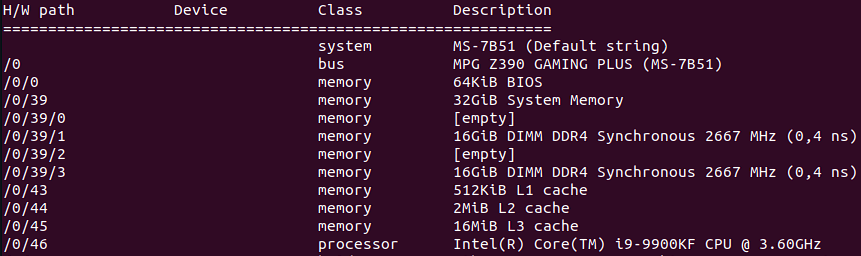
\includegraphics[scale=0.6]{images/Uni_Prozessor.PNG}
	\caption{Systeminformationen Laborrechner}
\end{figure}
Der ICS Mini II verfügt über einen Cortex A9 1Ghz Prozessor und über 1GB Arbeitsspeicher, in Abbildung 3 zu sehen.
\begin{figure}[H]
	\centering
	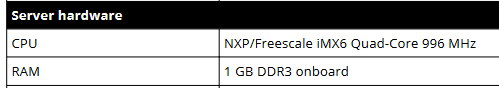
\includegraphics[scale=0.8]{images/Iseg_Prozessor.PNG}
	\caption{Systeminformationen ICS Mini II}{Quelle: \url{https://iseg-hv.com/files/media/iseg_manual_iCSmini2_en_20201023133528.pdf} Stand: 09.07.2022}
\end{figure}
\noindent
Mithilfe des Linux Befehls \enquote{time}\footnote{\url{https://man7.org/linux/man-pages/man1/time.1.html} Stand: 09.07.2022} wurden die Verifizierverfahren 100 mal ausgeführt, um daraus einen Mittelwert bilden zu können.
\subsection{C}
Zunächst sollen die Ergebnisse des Laborrechners dargestellt werden. Für das Verifizieren mit der Implementierung in C benötigte der Rechner 46,575 Sekunden, das entspricht 0,46576 Sekunden pro Verifizierung.
\begin{figure}[H]
	\centering
	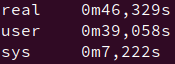
\includegraphics[scale=0.8]{images/Laborrechner_C.PNG}
	\caption{Zeit Laborrechner C}
\end{figure}
\noindent
Das Verifizieren mit GPG kostete den Laborrechner ganze 55,415 Sekunden, was wiederum 0,55415 Sekunden pro Verifizierung entspricht.
\begin{figure}[H]
	\centering
	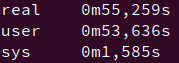
\includegraphics[scale=0.8]{images/Laborrechner_GPG.PNG}
	\caption{Zeit Laborrechner GPG}
\end{figure}
\subsection{GPG}
\noindent
Nun werden die Zeiten des ICS Mini II aufgezeigt. Für das Verifizieren mit der C Implementierung brauchte der ICS Mini II ... Sekunden, das entspricht ... Sekunden pro Verifizierung.
\begin{figure}[H]
	\centering
	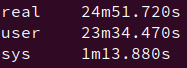
\includegraphics[scale=0.8]{images/ICS_MINI_C_100.PNG}
	\caption{Zeit ICS MINI II C}
\end{figure}
Das Verifizieren mit GPG dauerte 12 Minuten und 18,602 Sekunden mit dem ICS Mini II. Diese Zeit ergibt eine durchschnittliche Ausführungszeit von 7,38602 Sekunden pro Verifizierung.
\begin{figure}[H]
	\centering
	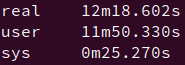
\includegraphics[scale=0.8]{images/ICSMINIII_GPG.PNG}
	\caption{Zeit ICS Mini II GPG}
\end{figure}
\newpage
\section{Ergebnis}
Das Verifizieren mit GPG schließt mit 7 Sekunden in einem passablen Zeitumfang ab. Dennoch würden 7 Sekunden eine merkbare Wartezeit im Aktualisierungsprozess darstellen. Eine mögliche Optimierung findet sich in der C-basierten Implementierung. Diese nimmt zwar im Durchschnitt 14-15 Sekunden in Anspruch, könnte aber wahrscheinlich verbessert werden. 13 Sekunden werden allein für das Hashen der Aktualisierungsdatei verwendet. Ein Austauschen des Hashingalgorithmus SHA-512 durch eine Implementierung von SHA-512 in ARMv7 Assembler könnte hier Abhilfe schaffen. Es ist unklar, ob damit der Verifiziervorgang auf unter 7 Sekunden gebracht werden könnte, aber es ist die beste Möglichkeit.
\\[1cm]
Zum derzeitigen Stand wäre die Umsetzung mit GPG die schnellste Lösung und wird somit mit großer Wahrscheinlichkeit auch Anwendung finden.
\section{Verwendung durch den Nutzer}
Es sollte diskutiert werden, wie Aktualisierung, Signatur und public-key künftig beim Nutzer ankommen. Die Aktualisierung wurde bisher standardmäßig online\footnote{\url{https://iseg-hv.com/en/products/control} Stand: 13.07.2022} zum Download angeboten. Mehrere Ideen stehen hierfür im Raum. Beim GPG Verfahren muss zudem der public-key als vertrauenswürdiger Schlüssel eingerichtet sein. Dies könnte auch automatisch beim Aktualisieren geschehen und erfordert nicht zwingend eine Aktion des Nutzers. Alle Vorschläge, welche einen public-key spezifisch ansprechen, thematisieren eine Implementierung in C.
\\[1cm]
Zunächst könnten Signatur und public-key im selben Downloadverzeichnis, wie bisher die Aktualisierung, angeboten werden. So würde es auf den Nutzer zurückfallen, sich bewusst die Signatur zu beschaffen. Würde er dies nicht, so würde die Aktualisierung auch ohne Signatur funktionieren, jedoch dann auf Risiko des Nutzers. Für ein Verfahren mit Verifizierung muss dem Nutzer eine einfache Möglichkeit im Webinterface geboten werden, um die Signatur und den Public Key im Update-Verzeichnis (/mnt/user/data/updates) zu hinterlegen und das Update-Skript mit entsprechenden Parametern aufgerufen werden.
\\[1cm]
Des Weiteren besteht die Möglichkeit, sämtliche benötigten Dateien in einem Tarball anzubieten. Dieser könnte heruntergeladen und vom Update-Skript vor der Installation entpackt werden. Somit müsste sich der Kunde nur um eine Datei aktiv kümmern, der Rest geschieht automatisch. Diese Möglichkeit würde allerdings die verifizierte Aktualisierung auf den Nutzer forcieren, da die Signatur automatisch verarbeitet wird. Hier müsste gegebenenfalls ein Input des Nutzers angefordert werden, ob er die Aktualisierung gegen die Signatur prüfen will.
\\[1cm]
Durchaus vorstellbar wäre auch die Signatur und Aktualisierung im GPG Signaturverfahren zu einer \enquote{.gpg}-Datei zu kombinieren. Vorteil dieser Methode ist, dass der Kunde nur, wie gewohnt, eine Datei herunterladen muss. Allerdings wird so ein Verifizieren erzwungen, da die \enquote{.gpg}-Datei vorher nicht als Aktualisierung genutzt werden kann. Dies könnte zu Problemen führen, falls ein Kunde keine Verifizierung möchte. Außerdem besteht die Möglichkeit, dass ein Kunde seine ICS Version so weit herunterstuft, dass er kein GPG mehr auf dem Gerät zur Verfügung hat. In solch einem Fall muss ein Update auch in ursprünglicher Form zum Download bereitstehen und nicht nur als \enquote{.gpg}-Datei.
\\[1cm]
Es könnte sich anbieten, bei erfolgreicher Verifizierung eine Art Flag in einer Log-Datei zu hinterlassen. Somit könnte gegen Nutzer vorgegangen werden, welche die Schuld für ihr nicht funktionierendes System in einer fehlerhaften Aktualisierung suchen. Wäre dieses Flag gesetzt, müsste die Installation mit einer unversehrten Datei abgelaufen sein und das System einwandfrei laufen (vorrausgesetzt, die Aktualisierung war nicht von vorneherein fehlerhaft).
So kann nur der Nutzer Schuld sein.
\section{Ausblick}
Eine Signatur im Ed25519-Signaturverfahren bietet derzeit ausreichend Schutz für das Sicherstellen der Integrität einer Iseg Firmwareaktualisierung. Dieser Schutz ist gegeben durch das Problem des diskreten Logarithmus. Der public-key lässt sich relativ leicht durch diskrete Epxonentiation aus einem private-key zu errechnen. Für die Umkehrfunktion der diskreten Exponentialfunktion, den diskreten Logarithmus, ist jedoch kein effizienter Algorithmus zur Berechnung bekannt. Dies macht es einem Angreifer sehr schwer, den private-key zu ermitteln. Er müsste mit den besten bekannten Algorithmen einen Aufwand von \begin{math}O(2^{128})\end{math} \footnote{\raggedright High-speed high-security signatures, \url{https://ed25519.cr.yp.to/ed25519-20110926.pdf}, S. 1, Stand: 12.07.2022} erbringen, um möglicherweise den private-key zu ermitteln. Für unseren Anwendungsfall ist es unwahrscheinlich, dass ein Angreifer genügend Rechenleistung aufbringen kann um dies in einem sinnvollen Zeitraum durchzuführen. Durch Wechseln des private-keys für jede neue Firmware-Version könnte dies noch weiter erschwert werden.
\\[1cm]
Sollte ein Quantencomputer mit ausreichend Anzahl an Qubits entwickelt werden, so wäre das Signieren mit Ed25519 nichtig, da mithilfe des Shor-Algorithmus \cite{SHOR} für Quantencomputer das oben genannte Problem trivialisiert werden kann. In diesem Fall bietet sich ein Umstieg auf symmetrische Signaturverfahren an, deren Sicherheit nicht durch die Existenz eines Quantencomputers beeinträchtigt ist. Als Beispiel lässt sich dafür AES-256 aufführen.

\appendix % Anhang	
\chapter{C Programmcode}
\section{Schlüsselerstellung und Signieren}
\begin{lstlisting}[language=C]
#include "ed25519.h"
#include <stdio.h>
#include <stdlib.h>
#include <string.h>
int main(int argc, char *argv[]) {

unsigned char seed[32], public_key[32], private_key[64], signature[64];
long FILE_SIZE;
char *BUFFER;


// open update file and read it into a BUFFER

FILE *UPDATE_FILE = fopen ( argv[1], "rb" );
if ( !UPDATE_FILE ) perror(argv[1]), exit(1);

fseek( UPDATE_FILE , 0L , SEEK_END);
FILE_SIZE = ftell( UPDATE_FILE );
rewind( UPDATE_FILE );
BUFFER = calloc( 1, FILE_SIZE + 1 );
if ( !BUFFER ) fclose(UPDATE_FILE), fputs("memory alloc fails", stderr), exit(1);

if ( 1 != fread( BUFFER , FILE_SIZE, 1 , UPDATE_FILE) )
fclose(UPDATE_FILE), free(BUFFER), fputs("entire read fails", stderr), exit(1);
fclose(UPDATE_FILE);

// write update file from BUFFER to char array

unsigned char *message = malloc(FILE_SIZE + 1 );

if (message == NULL) {
printf("error while allocating memory for update file");
free(BUFFER);
exit(1);
}

for (int i = 0; i < FILE_SIZE; ++i) {
message[i] = ((char *)BUFFER)[i];
}

free(BUFFER);

if (ed25519_create_seed(seed)) {
printf("error while generating seed\n");
exit(1);
}

ed25519_create_keypair(public_key, private_key, seed);

ed25519_sign(signature, message, FILE_SIZE, public_key, private_key);

free(message);


/*  splitting key creation and signing process:
- after ed25519_create_keypair, write public_key and private_key to any file
- in a separate program (signing) : load public_key private_key and the update file ("message") into char arrays
- file size of the update file and an empty 64 Byte char array (signature) are needed
- call ed25519_sign and pass the prepared parameters
- write public_key and signature to any file
- file size should be 96 Byte (32 Byte public_key + 64 Byte signature in that specific order)
*/

// write signature and public key to given file

FILE *KEY_SIG_FILE = fopen(argv[2], "wb+");
if (KEY_SIG_FILE == NULL)
{
printf("error opening file\n");
exit(1);
}
for (int i= 0; i < sizeof(public_key); i++) {
fputc(public_key[i], KEY_SIG_FILE);
}
for (int i= 0; i < sizeof(signature); i++){
fputc(signature[i], KEY_SIG_FILE);
}

fclose(KEY_SIG_FILE);

return 0;
}	
\end{lstlisting}
\section{Verifizieren}
\begin{lstlisting}[language=C]
#include "ed25519.h"
#include <stdio.h>
#include <stdlib.h>
#include <string.h>
#include <time.h>
int main(int argc, char** argv) {

// public key has to be 32-Byte writable char array
// signature has to be 64-Byte writable char array

long FILE_SIZE;
char *BUFFER;
unsigned char PUBLIC_KEY[32], SIGNATURE[64];


// load public key and signature

FILE *SIGNATURE_FILE = fopen ( argv[2] , "rb" );
if ( !SIGNATURE_FILE ) {
perror(argv[2]), exit(1);
}

fseek( SIGNATURE_FILE , 0L , SEEK_END);
FILE_SIZE = ftell( SIGNATURE_FILE );

// "SIGNATURE_FILE" has to be 96 Bytes ((public_key)32+64(signature))
if (FILE_SIZE != sizeof(PUBLIC_KEY)+sizeof(SIGNATURE)) fclose(SIGNATURE_FILE), fputs("incompatible signature type\n", stderr), exit(1); 

rewind( SIGNATURE_FILE );

BUFFER = calloc( 1, FILE_SIZE + 1 );
if ( !BUFFER ) fclose(SIGNATURE_FILE), fputs("memory alloc fails", stderr), exit(1);

if ( 1 != fread( BUFFER , FILE_SIZE, 1 , SIGNATURE_FILE) )
fclose(SIGNATURE_FILE), free(BUFFER), fputs("entire read fails", stderr), exit(1);
fclose(SIGNATURE_FILE);

// write public key and signature to respective variables

for (int i = 0; i < FILE_SIZE; ++i) {
if ( i < sizeof(PUBLIC_KEY)) {
PUBLIC_KEY[i] = ((char *)BUFFER)[i];
}
else 
SIGNATURE[i-sizeof(PUBLIC_KEY)] = ((char *)BUFFER)[i];
}

free(BUFFER);

// load update file

FILE *UPDATE_FILE = fopen ( argv[1], "rb" );
if ( !UPDATE_FILE ) perror(argv[1]), exit(1);

fseek( UPDATE_FILE , 0L , SEEK_END);
FILE_SIZE = ftell( UPDATE_FILE );
rewind( UPDATE_FILE );

BUFFER = calloc( 1, FILE_SIZE + 1 );
if ( !BUFFER ) fclose(UPDATE_FILE), fputs("memory alloc for reading in the update file failed", stderr), exit(1);

if ( 1 != fread( BUFFER , FILE_SIZE, 1 , UPDATE_FILE) )
fclose(UPDATE_FILE), free(BUFFER), fputs("reading of update file failed", stderr), exit(1);
fclose(UPDATE_FILE);

unsigned char *message = malloc(FILE_SIZE + 1 );

if (message == NULL) {
printf("error while allocating memory for update file");
free(BUFFER);
exit(1);
}

for (int i = 0; i < FILE_SIZE; ++i) {
message[i] = ((char *)BUFFER)[i];
}
free(BUFFER);

// verify integrity of update file

if (ed25519_verify(SIGNATURE, message, FILE_SIZE, PUBLIC_KEY)) {
printf("\nvalid signature\n");
return 0;
} else {
printf("\ninvalid signature\n");
return 1;
}
free(message);


}
\end{lstlisting}
\chapter{Bash Programmcode}
\section{Variablendeklaration}
\begin{lstlisting}[language=bash]
GPG=`command -v gpg` || { echo >&2 "Update ERROR: Program gpg not available.  Aborting."; exit 1; }
	
	# START
	
	ZIP_FILE_PATH="/mnt/user/data/updates/"
	ZIP_FILE=""
	GPG_SIG_FILE=""
	C_SIG_FILE=""
	C_VERIFY_FILE="verify_file_arm"
	IS_VALID_SIGNATURE=""
	while getopts "nrRhf:p:g:Gs:S:C:" Option ; do
		case $Option in
			n)	NO_RECURSE=1
				;;
			r) 	FactoryReset
				exit 0
				;;
			R) 	FactoryReset full
				exit 0
				;;
			h) 	Usage
				# Exit if only usage (-h) was specfied.
				if [ "$#" -eq 1 ] ; then
					exit 10
				fi
				exit 0
				;;
			f)	ZIP_FILE=$OPTARG
				;;
			p)	ZIP_FILE_PATH=$OPTARG
				;;
			g)	ISEG_SERIAL=$OPTARG
				GetDeviceType ${ISEG_SERIAL}
				exit 0
				;;
			G)	GetDefaultDeviceType
				exit 0
				;;
			s)	SET_CONFIGURATION=$OPTARG
				SetConfiguration "/" ${SET_CONFIGURATION}
				exit 0
				;;
			S)	GPG_SIG_FILE=$OPTARG
				;;
			C)	C_SIG_FILE=$OPTARG
				;;
		esac
	done
	
	if [ "$ZIP_FILE" = "" ] ; then
		Usage
		exit 0
	fi
	
	# is ZIP_FILE an existing file?
	if [ ! -r "${ZIP_FILE_PATH}${ZIP_FILE}" ] ; then
		echo >&2 "Update ERROR: ${ZIP_FILE_PATH}${ZIP_FILE} does not exist or cannot be read, exiting"
		exit 1
	fi	
\end{lstlisting}
\section{Verifizieren mit GPG}
\begin{lstlisting}[language=bash]
# is ZIP_FILE a signed GPG file? (non detached signature)
	if [ "${ZIP_FILE: -4}" == ".gpg" ] ; then
	
		echo "checking signature..."
		${GPG} --yes --output "${ZIP_FILE_PATH}${ZIP_FILE%.gpg}" --decrypt "${ZIP_FILE_PATH}${ZIP_FILE}" 2>/dev/null
		IS_VALID_SIGNATURE=$?
	
		if [ $IS_VALID_SIGNATURE -eq 1 ] ; then
			echo "incorrect GPG signature, check the signature file name for errors: ${ZIP_FILE_PATH}${ZIP_FILE}"
			exit 1
		elif [ $IS_VALID_SIGNATURE -eq 2 ] ; then
	        	echo "invalid GPG signature, check the signature file name for errors: ${ZIP_FILE_PATH}${ZIP_FILE}"
	        	exit 1
	    	else
	    		ZIP_FILE=${ZIP_FILE%.gpg}
	    		echo "correct signature, resuming update..."
	    	fi
	fi
	
	# if a GPG_SIG_FILE was provided, check if it is a valid GPG signature
	if [ -f "${ZIP_FILE_PATH}${GPG_SIG_FILE}" ] ; then
	
		if [ "${GPG_SIG_FILE: -4}" == ".gpg" ] ; then
			echo "pass .gpg files only as argument to the -f parameter"
			exit 1
		fi
	
		echo "checking signature..."
		${GPG} --verify "${ZIP_FILE_PATH}${GPG_SIG_FILE}" "${ZIP_FILE_PATH}${ZIP_FILE}" 2>/dev/null
		IS_VALID_SIGNATURE=$?
	
		if [ $IS_VALID_SIGNATURE -eq 1 ] ; then
			echo "incorrect GPG signature, check the signature file name for errors: ${ZIP_FILE_PATH}${GPG_SIG_FILE}"
			exit 1
	
		elif [ $IS_VALID_SIGNATURE -eq 2 ] ; then
	       		echo "invalid GPG signature, check the signature file name for errors: ${ZIP_FILE_PATH}${GPG_SIG_FILE}"
	        	exit 1
	    	else
			echo "correct signature, resuming update..."
		fi
	fi	
\end{lstlisting}
\newpage
\section{Verifizieren mit C Implementierung}
\begin{lstlisting}[language=bash]
# if a C_SIG_FILE (signature generated by ed25519 c program) was provided, check if it is a valid signature
	if [ -f "${ZIP_FILE_PATH}${C_SIG_FILE}" ] ; then
	
		echo "C checking signature..."
		${ZIP_FILE_PATH}${C_VERIFY_FILE} ${ZIP_FILE_PATH}${ZIP_FILE} ${ZIP_FILE_PATH}${C_SIG_FILE}
		IS_VALID_SIGNATURE=$?
	
		if [ $IS_VALID_SIGNATURE -eq 1 ] ; then
			echo "invalid signature, check the signature file name for errors: ${ZIP_FILE_PATH}${C_SIG_FILE}"
			exit 1
		else
			echo "correct signature, resuming update..."
		fi
	fi
	exit 0
\end{lstlisting}
\bibliographystyle{plain}
\bibliography{refs.bib}
\end{document}